\section{Performance Benefits}
\label{sec:perf}

%We now present some initial benchmarks and results to justify the
%feasibility of our vision.
In this section, we use a custom simulator to compare the
performance of our FSO-based architecture(s) against state-of-art  \DC
designs.   As a representative point, we consider a \DC with 24,576
machines organized into 512 racks of 48 machines. Our results are
qualitatively similar for other configurations.


\begin{table}[t]
\begin{small}
\begin{center}
\begin{tabular}{c|c|c}
%\hline
Architecture & Cost (\$) & Effective per-server throughput \\   \hline % \hline
FSO-based (16,5) & 18.1M  & 1.7 Gbps\\    %\hline
3D Beamforming & 17.1M  & 1.1 Gbps\\% \hline
Fattree/Jellyfish 1Gbps & 13M & 1 Gbps\\%   \hline
Fattree/Jellyfish 2 Gbps & 26M  & 2 Gbps \\ \hline
FSO (48,10) & 37.8M  & 8.5 Gbps \\ %\\   \hline
Fattree/Jellyfish 10Gbps & 57M  & 10 Gbps%\\   \hline
\end{tabular}
\end{center}
\end{small}
\vspace{-0.3cm}
\tightcaption{Cost-performance tradeoffs for 512 racks with 48 machines/rack:
 The FSO designs are specified by (\#FSOs, \#SMs/FSO).}
\vspace{-0.3cm}
\label{table:cost}
\end{table}

\para{Candidate Architectures and Costs.}
 The specific architectures we consider 
are:\footnote{We don't consider the all-wireless architecture
of~\cite{cornell} because  it has
worse cost-performance tradeoffs relative to the below
architectures; e.g., for 24k machines, it costs $\approx 50M$ (based on \$1k for a 60GHz radio) 
but only achieves 300-400 Mbps per-server and has an
average/max. hop-count of about 10/100~\cite{cornell}.}

\begin{packeditemize}
\item {\bf Fat-tree~\cite{fattree}:} We consider
   1Gbps and 2Gbps bisection-bandwidth FatTree networks. A
  2Gbps network is essentially two 1Gbps networks put together.

\item {\bf Jellyfish~\cite{jellyfish}:} We construct wired random
graphs~\cite{jellyfish} and similar to FatTree, we consider both 1 and 2~Gbps
architectures.

\item {\bf 3D-Beamforming~\cite{3db}:} We use a wired 1Gbps
  bisection-bandwidth network augmented with eight 60GHz wireless
  radios per rack~\cite{3db}. We conservatively assume 0.01s antenna
  rotational delay (lower bound from~\cite{3db}), no interference, and
  a 1-10~Gbps bandwidth for wireless links based on inter-rack
  distances~\cite{3db}.

\item {\bf FSO-based designs:} We use two pre-configured topologies
  (\S\ref{sec:pre-conf}): (1) {\tt Random} and (2) {\tt Hypercube+}.
  We use a 64-port 10Gb ToR switch~\cite{64switch}; 48 ports
  connect to machines and 16 ports  to FSO devices.
  Each FSO link is 10~Gbps, since we use 10Gbps optical SFPs as
  our cost basis.  We assume each FSO device has 5 SMs,
  with a switching latency of 20~ms.
%and  also study   the effect of varying this, a SM switching latency of 20~ms.
%\blue{Based on our experiment, we    use a switching latency of 20 msec.}
\end{packeditemize}

Ideally, we want to compare architectures by normalizing their cost.
Unfortunately, some architectures (e.g., Fat-tree, {\tt Hypercube+})
do not admit a continuous spectrum of cost-performance
tradeoffs. Further, some of these cost estimates are moving targets.
As such, we pick configurations where the costs are roughly comparable
based on estimates we obtain as discussed below.

We assume that a 64-port 10Gb ToR switch for the FSO designs costs
\$27K: \$11K for the bare switch~\cite{64switch}, and \$16K for 64
10Gbps optical SFP+ transceivers at \$250 each~\cite{sfp}. We assume
that a 48-port 1Gb switch costs \$5000~\cite{48-switch-cost}, and each
60GHz radio costs \$1000. From \S\ref{sec:fso}, each FSO device costs
an additional $\approx$ \$500 with \$5 for a small-size SM, when
manufactured at scale~\cite{sm-personal}.  We assume ceiling mirrors
(for FSO and 3D-beamforming) have negligible cost and we
conservatively ignore cabling costs for the wired architectures. Given
the above assumptions, Table~\ref{table:cost} summarizes the costs.
Here, Fat-tree/Jellyfish 1Gbps use  2600 48-port 1Gb switches. We
see that FSO-based designs roughly fall between the 1~Gbps and 2~Gbps
wired architectures. As additional points of reference, the table also
shows 10~Gbps architectures for FSO and Fat-tree (discussed later).

%\footnote{We do
 % not have access to real datacenter workloads and the public ones
  % that exist do not map data sources to rack locations.}

\begin{figure}[t]
\begin{center}
\subfloat[Uniform]
{
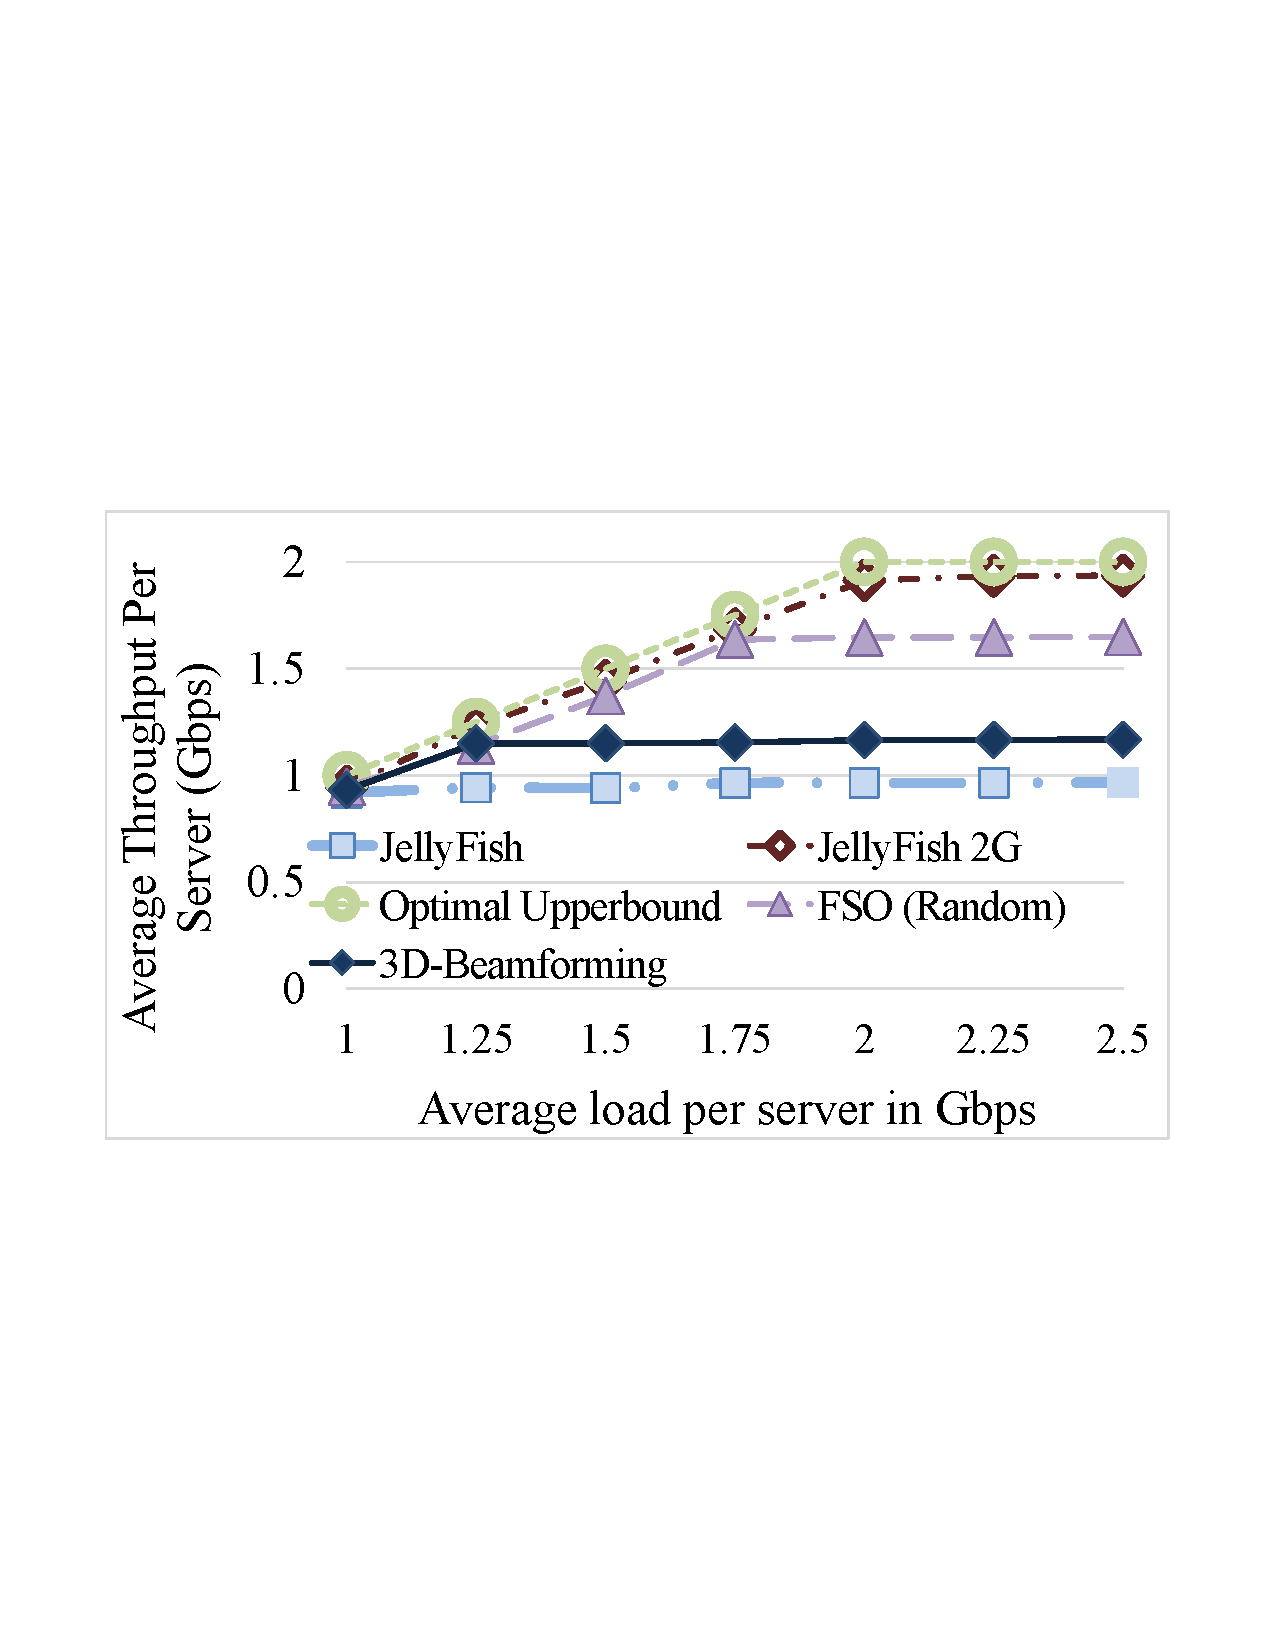
\includegraphics[width=180pt]{Figures/NewFigures/NormalTraffic.pdf}
} \\ \vspace{-0.3cm}
\subfloat[Hotspot]
{
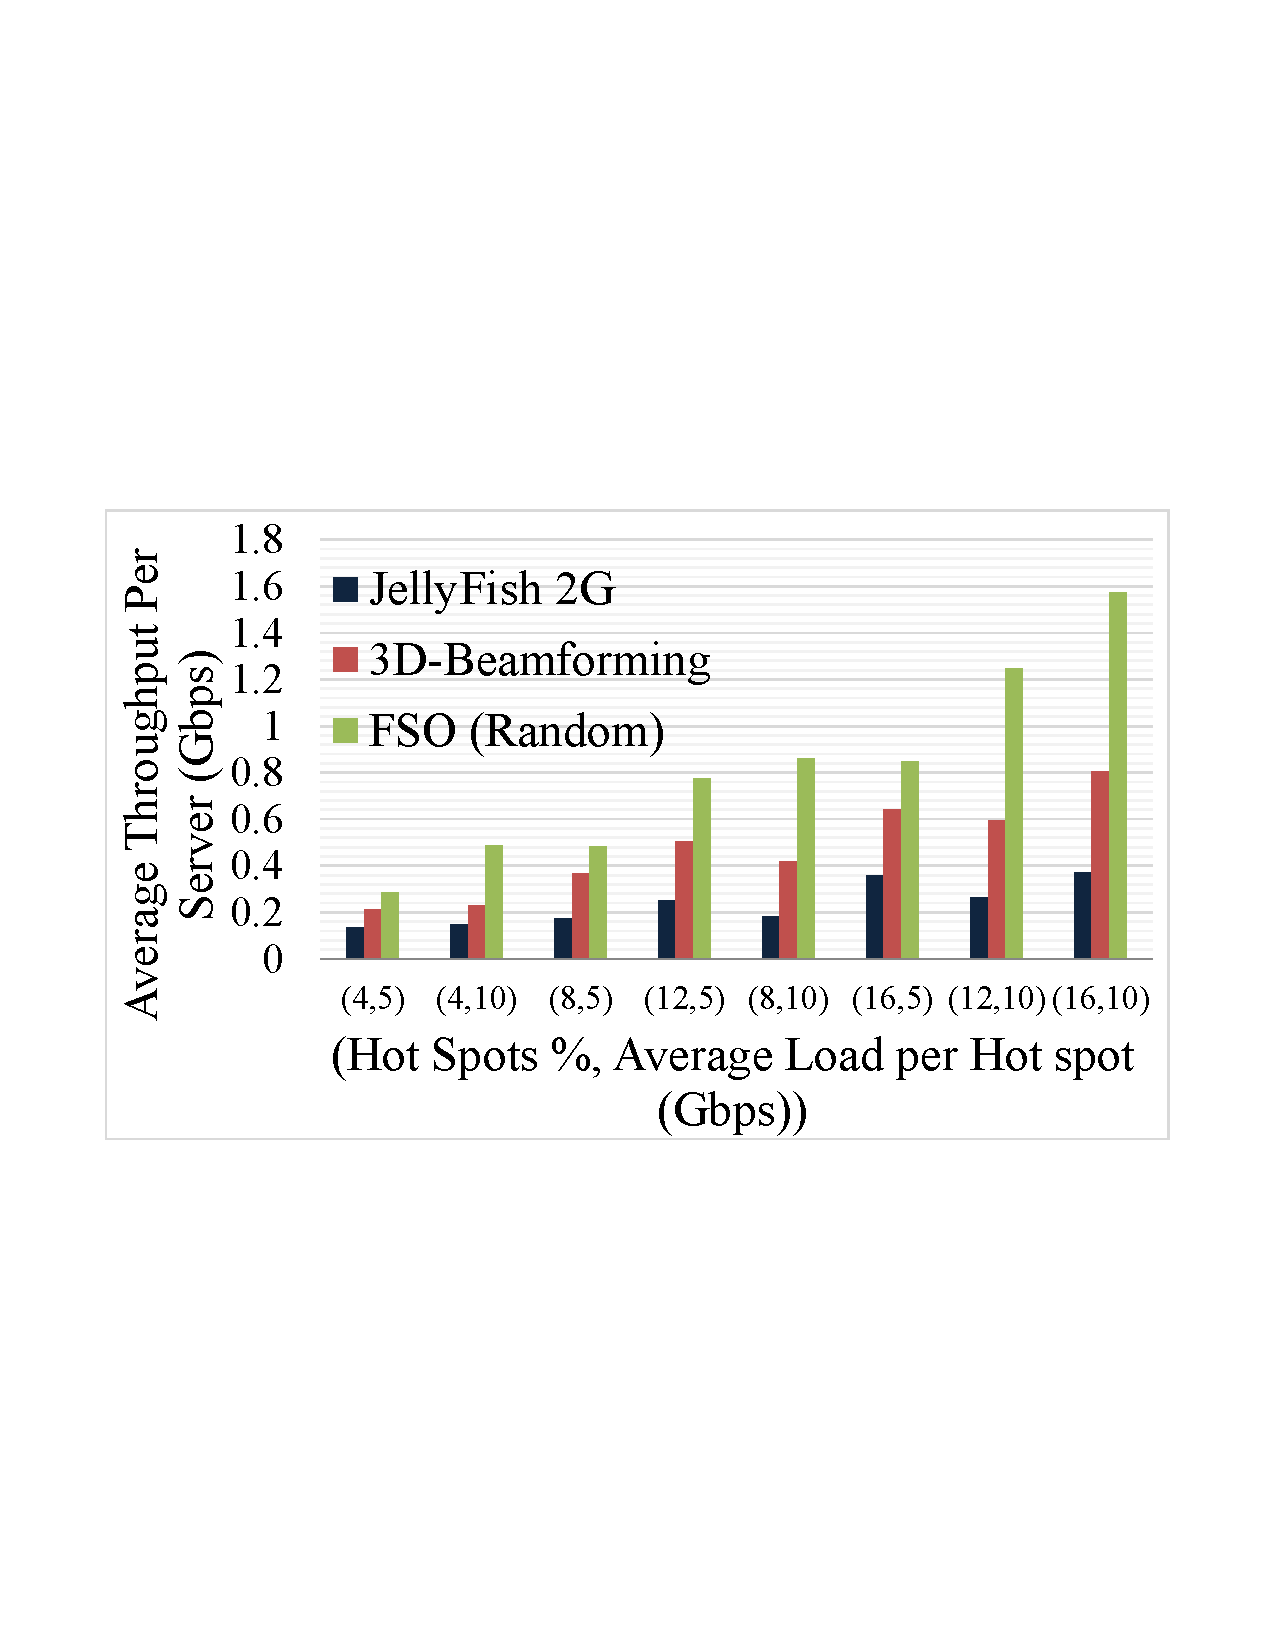
\includegraphics[width=180pt]{Figures/NewFigures/Hotspots.pdf}
}
\end{center}
\vspace{-0.3cm} \tightcaption{Average per-server throughput for the
  {\tt Uniform} and {\tt HotSpot} workloads.  The
  $x$-axis shows the average load per server which is a 
  product of arrival-rate (per pair), number of servers (512),
  and average flow size. The result for Hypercube+  is identical 
 to Random and the result for Fat-tree is identical to Jellyfish 
 and are not shown.}
\vspace{-0.3cm}
\label{fig:tput}
\end{figure}

\para{Simulation Setup.} For scalability, we consider 
   a flow-level simulation using a fluid model, and do not model 
 packet-level or TCP effects. 
% assuming} the buffer queue
%of each switch to be bounded (400MB) with the ``overflow'' packets
%being dropped.
 We use synthetic traffic models based on
prior measurement studies as follows~\cite{vl2,3db}.  We consider a
{\em baseline} workload where, for each pair of machines, flows arrive
independently based on a Poisson distribution with a {\em
  arrival-rate} $\lambda$/s, with the flow size distribution
measurements from production \DCs~\cite{vl2}.  We refer to
this as the {\tt Uniform} workload.  Prior studies have observed
hotspots between pairs of racks~\cite{vl2}; thus we consider the {\tt
  Hotspot} model where in addition to the {\tt Uniform} baseline, we
use a higher arrival-rate $\lambda_2$ and a fixed flow-size of 128MB
for a subset of machines chosen as follows~\cite{3db}. We randomly
pick $x$\% of machines, and for each one of them, we pick $x/2$\% of
machines as their destinations with a slight bias~\cite{3db}; we vary
$\lambda_2$ and $x$ in our simulations.  

\para{Throughput and Latency.}  Figure~\ref{fig:tput}(a), shows the average
per-server throughput for the {\tt Uniform} workload.  We observed that
Jellyfish and Fat-Tree architectures are nearly identical  and the two
FSO-based architectures (Random and Hypercube+) also have the same performance.
For ease of presentation,  we omit  plots for Fat-Tree and Hypercube+.

\begin{figure}[t]
\vspace{-0.3cm}
\begin{center}
%\begin{tabular}{cc}
\subfloat[Vary \#SMs]
{
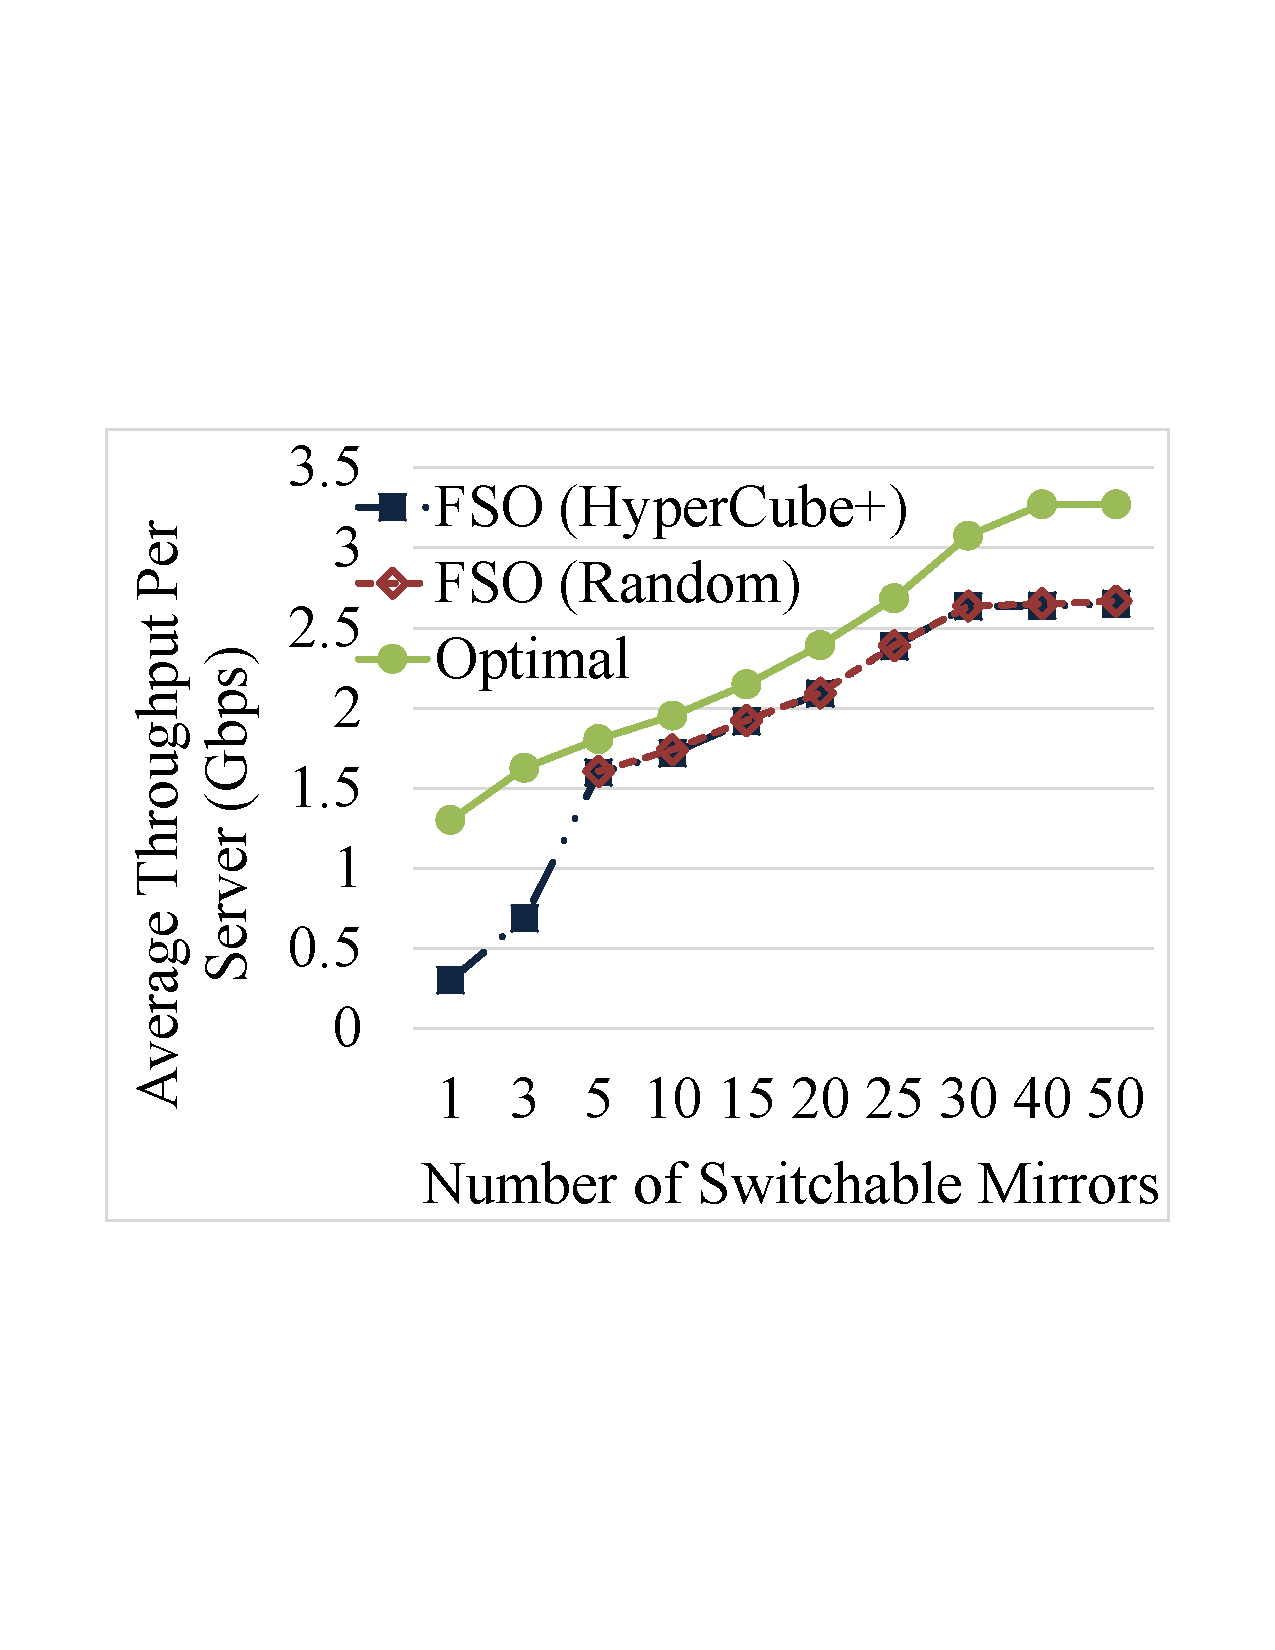
\includegraphics[width=0.22\textwidth]{Figures/NewFigures/Mirrors.pdf}
}
\subfloat[Vary \#FSOs]
{
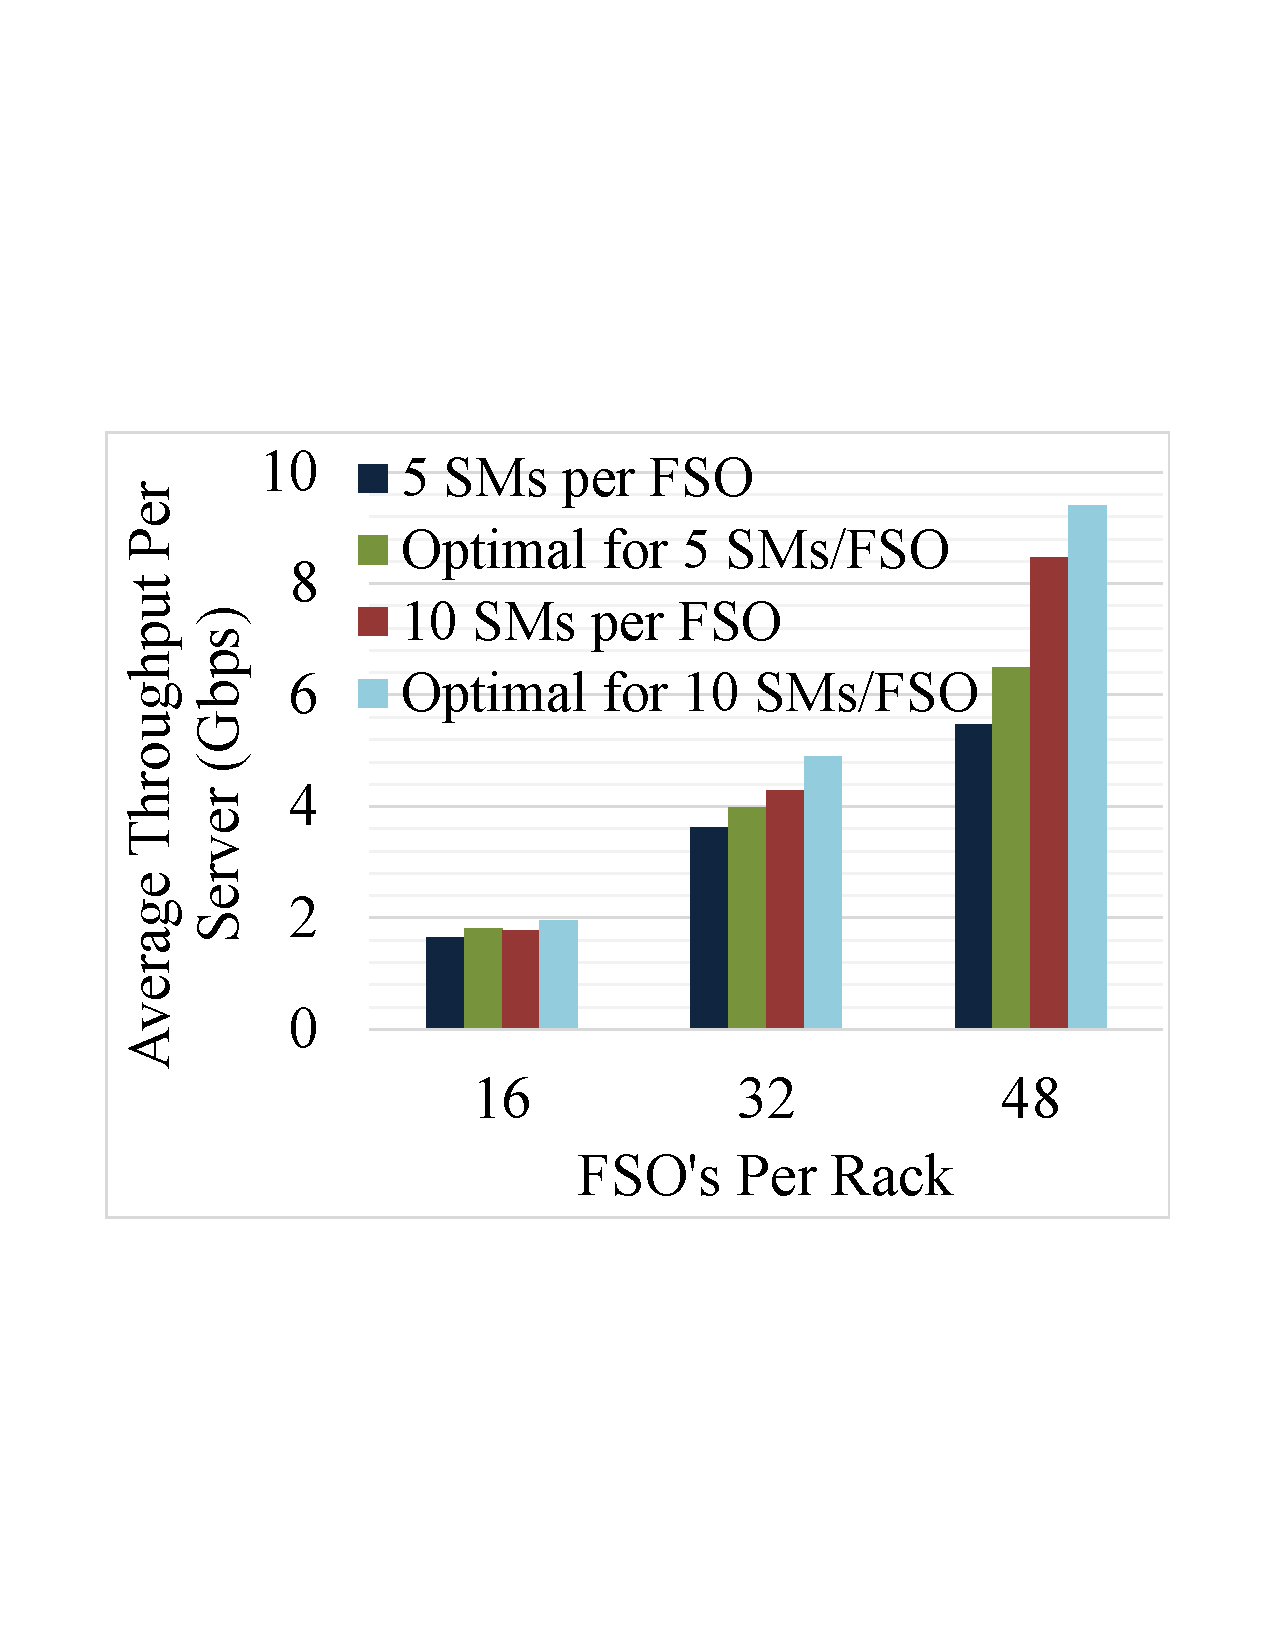
\includegraphics[width=0.22\textwidth]{Figures/NewFigures/FSOMirrors.pdf}
}
%\end{tabular}
\end{center}
\vspace{-0.3cm}
\tightcaption{Sensitivity analysis,  varying number of FSOs and number of SMs using
 the baseline {\tt Uniform} workload}
% Average per-server throughput for various
%  configurations at {\em saturated} loads. (a) Varying number of SMs
%  per FSO, with 16 FSO per rack. (b) Varying number of FSOs per rack,
%  with 5 or 10 SMs per FSO.  Both experiments use a {\tt Uniform}
%  traffic, with an average server load of 5Gbps and 20Gbps
 % respectively.}
\label{fig:sms}
\end{figure}

We see that FSO-based architectures provides 1.7Gbps of average
throughput per server, which is significantly higher than 1Gbps
Jellyfish/Fattree and 3D-Beamforming, but slightly lower than the
2Gbps Jellyfish/Fattree.  As a point of reference, we compute an
upper bound on the {\em optimal} throughput achievable with FSOs. Given
a configuration of \# FSOs per rack and \# SMs per FSO, we compute
this bound by estimating the minimum possible average shortest-path
length; we omit the details due to space limitations. We see that our
design performs quite close to the upper-bound of $\approx$ 2Gbps.

For the {\tt HotSpots} workload in Figure~\ref{fig:tput}(b), as
in~\cite{3db} we use a low baseline load of 0.1Gbps average load per
server.\footnote{We also tried other baseline loads. FSO
  outperforms other solutions under all scenarios, but the relative gain
  decreases at higher load as there is less scope for
  improvement.}  We consider different configurations for the number
of hotspots and intensity (i.e., $x\%$, average load per hotspot) as
shown. First, we see that all flexible architectures (FSO-based and
3D-Beamforming) outperform the static Jellyfish (and Fat-Tree) 2Gbps
designs.  Second, the FSO-based design outperforms 3D-beamforming by
large margin (30 to 100\%).

We also measured the latency in terms of inter-rack hops per-packet.
The average, 95\%ile, and max latency for FSO-based proposals were
2.5, 6, and 12 hops respectively (not shown). In comparison, the
corresponding numbers for Fat-tree and Jellyfish are 3.9,4,4 and
 2.5, 3, 5 hops respectively. We see that in the common case, FSOs
provide low latency, but in some very rare cases we incur longer
paths.

% (For reference, the 95\%ile latency for FSO is 6 hops which is
% comparable to the max for others).

% \vyas{is this inter rack or inter machine .. also show fattree or jellyfoish as point of reference}

\para{Sensitivity Analysis.} The previous results consider a fixed number of
FSOs per rack and SMs per FSO device. In Figure~\ref{fig:sms}, we vary (a) the
number of SMs keeping the number of FSOs at 16/rack, and (b) the number of
FSOs per rack for 5 and 10 SMs/FSO.  (We do not show  {\tt Random} for less
than 5 SMs, since it does not form a connected graph.) First, we see that the
effective per-server bandwidth increases with the increase in SMs, but
saturates at around 30 SMs per rack (when we almost get a complete candidate
graph).  Second, the configuration of 48 FSOs with 10 SMs provides almost
8.5Gbps. 

Given our current size estimates, it is actually feasible to place 48
FSOs on each rack; the total cost of this architecture is $\approx$
\$38M.  We estimate this assuming a 96-port 10Gb switch (hypothetically)
costs \$49k (= \$25k for the  switch + cost for 96 SFP+ modules at \$250
each).  In comparison, a 10Gbps Fat-tree architecture would
(conservatively) cost around \$57M assuming each 48-port 10Gb switch
costs \$22k (= \$10k~\cite{48-10-switch} + cost for 48 SFP+ modules).
